\documentclass{standalone}
\usepackage{tikz}
\usepackage{ctex,siunitx}
\setCJKmainfont{Noto Serif CJK SC}
\usepackage{tkz-euclide}
\usepackage{amsmath}
\usepackage{wasysym}
\usetikzlibrary{patterns, calc}
\usetikzlibrary {decorations.pathmorphing, decorations.pathreplacing, decorations.shapes,}
\begin{document}
\small
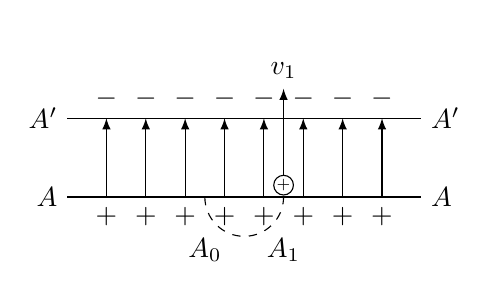
\begin{tikzpicture}[>=latex,scale=0.5]
  \useasboundingbox(-1,4.3)rectangle(10,-2);
  \draw (0,0)node [left]{$A$}--(9,0)node [right]{$A$};
  \draw (0,2)node [left]{$A'$}--(9,2)node [right]{$A'$};
  
  \foreach \x in {1,2,...,8}
  {
      \draw [->](\x,0)--(\x,2);
     \node at (\x, 2.5){$-$};  \node at (\x, -.5){$+$};
  }
  \draw [dashed] (3.5,0) arc (180:360:1);
  
  
  \draw (5.5,.3) circle (.25) node {\tiny +};
  
  \draw [->](5.5,.55)-- (5.5,2.75)node[above]{$v_1$};
  \node at (3.5,0)[below=4mm]{$A_0$};
  \node at (5.5,0)[below=4mm]{$A_1$};
\end{tikzpicture}
\end{document}